% 度量空间
% 度量空间|欧几里得空间|距离函数

\begin{definition}{度量空间}
一个集合中任意两个元素 $u, v$ 间若定义了满足以下条件的\textbf{距离函数(distance function)} $d(u, v)$, 那它就是一个\textbf{度量空间}. 集合中的每个元素就叫空间中的一个\textbf{点}.
\begin{itemize}
\item $d(u, u) = 0$
\item $d(u, v) > 0$
\item $d(u, v) = d(v, u)$
\item $d(u, v) \leqslant d(u, w) + d(w, v)$
\end{itemize}
\end{definition}

\begin{exercise}{欧几里得空间}
$N$ 维欧几里得空间 $\mathbb R^N$ 中若定义距离函数为
\begin{equation}
d(x, y) = \sqrt{\sum_{i=1}^N (x_i - y_i)^2}
\end{equation}
那么它是一个度量空间.
\end{exercise}

\begin{figure}[ht]
\centering
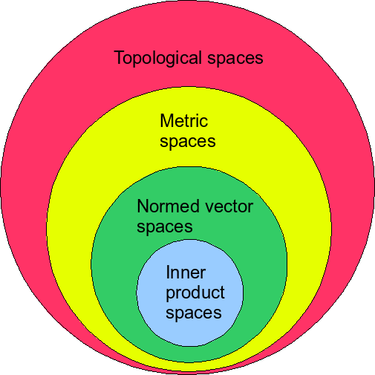
\includegraphics[width=6.5cm]{./figures/Metric1.png}
\caption{用维恩图表示几种不同空间之间的关系, 从内到外分别是内积空间\upref{InerPd}, 赋范空间\upref{NormV}, 度量空间, 拓扑空间(来自维基百科)} \label{Metric_fig1}
\end{figure}
